\chapter{ Perspectives}
\label{resultchapter}



%\section{Perspective}

\begin{itemize}

  \item \textbf{Hybrid Models / Dynamic Load Balancing Implementation / Computational Complexity Study} {
  
The idea of LES and filtering the velocity-field has been a breakthrough in numerical simulation of turbulence
yet still have some limitations including large computational cost for high-Reynolds number flows.
To overcome the LES shortcomings, there has been a considerable interest in development of hybrid turbulence models.
%Hybrid LES/RANS methods are a very active and interesting field of research in numerical fluid mechanics.
Since they aim at providing better results than RANS without the cost of a complete LES in the entire domain.
This is essential for many industrial applications, in particular for high-Reynolds number flows in the presence of walls.
%
The high compression property of the wavelet-based decomposition
is a promising feature which can make very large scale hybrid adaptive wavelet-based DNS/LES/URANS of turbulent flows a reality.
%
This work is an attempt develop a framework for
very large-scale parallel hybrid adaptive wavelet-based simulation of turbulence.
%
Two major building blocks required for such a framework are
1) hybrid models within the context of adaptive wavelet-based methods by means of the notion of defining the thresholding-factor of the wavelet
threshold filter as a field variable (spatial/temporal variable thresholding); and
2) highly-scalable parallel adaptive wavelet-based PDE solver.

%the spatial/temporal variable thresholding which is the infrastructure of hybrid models within the context of wavelet-based methods; and a highly-scalable parallel adaptive wavelet based PDE solver.




In wavelet based methods in general and particularly in SCALES,
implementation of Hybrid DNS/LES/RANS only requires change of wavelet thresholding-factor
with no additional efforts for merging two different solvers.
%
Because, within the context of wavelet-based methods, variable fidelity is achieved by changing the thresholding-factor:
very small thresholding-factor corresponds to WDNS,
moderately small thresholding-factor corresponds to CVS,
larger value of thresholding-factor along with solving the SGS models result in SCALES, and
much larger value of thresholding-factor for solving Unsteady Reynolds Averaged Navier-Stokes equations lead to
WURANS\cite{AIAA_2006} (wavelet-based URANS).
%
Hence, a careful combination of WDNS, CVS, SCALES, and WURANS in a systematic manner can lead to fully adaptive wavelet-based hybrid method.

Transition from WDNS to CVS is very straightforward since it can be controlled only by change of thresholding-factor. Transition from SCALES to CVS can be performed differently. Three main possibilities are:
1) Utilizing SGS model to control SGS dissipation (which has already been discussed) at all time throughout the entire spatial space;
2) instead of solving SGS model, at the CVS level, local kinetic energy of the last band can be monitored; and
3) instead of solving SGS model, at the CVS level, a virtual dissipation -- defined analogous to the SGS dissipation -- can be monitored.
%
Since most of the dissipation occur at the Kolmogorov scale, dissipation is more smooth and pronounced;
however, the kinetic-energy is more noisy at the Kolmogorov scale. This implies that dissipation can be a better measure to identify whether or not we are in the Inertial range, consequently the third (and first) approaches seem to be more practical. On the other hand, the second approach is easier to implement than the third method.
%Al in all
Therefore, first approach is the most realistic and easiest technique, in spite of the fact that it requires solving SGS equations at all times everywhere. As a result, transition from SCALES to CVS can also be defined based on change of thresholding-factor.

The transition from SCALES to WURANS is challenging since it requires switching between SGS models and turbulence models in addition to change of thresholding-factor. Although this can also be handled within one framework using the self-adapting turbulence models\cite{PetrotGadebusch_SelfAdaptingModel_POF_2007}.
The advantage of these kind of self-adapting models is that they are sufficiently powerful to model the turbulence
at any mesh resolution since the classic LES models based on the Smagorinsky approach are limited
to meshes that lie in the Inertial range. This is because
they all assume that the relevant length scale for the model is
the mesh size. In the inertial range this assumption holds, but
when the mesh is very coarse -- in the energy containing
range -- or very fine -- in the DNS range -- this assumption is
incorrect\cite{MeneveauLund_DynamicSmagorinskyModel__POF_1997}
and the classic LES approach and its variations like dynamic modeling are fundamentally flawed\cite{PetrotGadebusch_SelfAdaptingModel_POF_2007}.
%
Since SCALES is resolving the most energetic structures (either small- or large-scale), in case of using
local dynamic energy-based eddy-viscosity models, this problem is in fact less pronounced. %more based on the SGS models.
%
Within SCALES framework, due to self-adaptive nature of wavelets, different possibilities can be considered, like
a combination of both SGS models and turbulence models with some decaying function of thresholding-factor
as a multiplier for turbulence models to mimic their effects while thresholding is decreasing.

Therefore, it is evident that the main requirement for implementation of hybrid wavelet-based models
are the capability to dynamically change the thresholding-factor based on instantaneous flow realization. 
The idea of temporal/spatial varying thresholding has been proposed in the Chapter 2
and its promising initial results are demonstrated within the context of forced homogeneous turbulence in Chapter 3.
%
That is to say, the first aforementioned objective has already been developed. However, both large-scale simulations and large Reynolds numbers studies require scalable parallel code. Therefore, the main objective at the moment is to develop a parallel variable fidelity adaptive wavelet-based solver with hybrid models for both forced homogeneous turbulence and external flow applications.

The parallel algorithm for the adaptive wavelet collocation method and 
parallel integrated environment for variable fidelity adaptive multiscale modeling and simulation of turbulence
have already been developed in our group. 
%
Several partitioning approaches with different user controls are implemented (Figure ~\ref{fig:DifferentPartitioning}). More
advanced Zoltan\cite{ZoltanOverviewArticle,ZoltanHomePage,ZoltanUsersGuideV3,ZoltanDevelopersGuideV3,ZoltanHypergraphIPDPS06,ZoltanParHypRepart07}
library based partitions provide nearly optimal load balancing. In short, for
the geometric simultaneous partitioning all spatial directions of the domain are divided simultaneously.
The major deficiency of that approach is poor load balancing for a non-uniform
wavelet distribution. For the geometric sequential partitioning, the domain is subdivided by
planes normal to the first axis on rounded to the nearest integer $\sqrt[d]{P}$ sub-domains, where $d$ is
the problem dimension and $P$ is the total number of processors. The available $P$ processors
are distributed among these sub-domain according to the number of active wavelets inside
each of the sub-domains. This recursion step is repeated $d$ times to get the final partitioning.
It may deliver not quite an optimal load balancing, though it may be more usable for
non-uniform wavelet distributions across the domain. For significantly non-uniform wavelet
distribution, the domain is partitioned using Zoltan partitioning library by Sandia National
Laboratories (Figure ~\ref{fig:DifferentPartitioning}).



Dynamic load balancing is implemented via domain repartitioning during grid adaptation
step and reassigning tree data structure nodes to the appropriate processors. User provides
an imbalance tolerance vector to trigger the repartitioning if necessary. Depending on the
imbalance of wavelet distribution a different kind of repartitioning is performed. Highly
imbalanced data will be partitioned without considering initial decomposition, moderately
imbalanced repartitioned while trying to stay close to the current decomposition, and nearly
balanced will be refined by small changes only.
%
Three dimensional example of dynamic load balancing
for the 3D simulations of the Convection-Diffusion of rotating ellipsoids
is presented in Figure ~\ref{fig:ExamplePartitioning}.

The preliminary studies of the code scalability have been performed for
the CVS (thresholding-factor $\epsilon\rm{=0.2}$)
of linearly forced ($C_f\rm{=6.\bar{6}}$) homogeneous turbulence at $Re_{\lambda}=190$
on an adaptive grid corresponds to  $1024^3$ (at the highest level of resolution)
using geometric sequential partitioning (fixed partitioning), Figure ~\ref{fig:speedup}.
The scalability studies confirm that parallel code even without dynamic load balancing is scalable
with the speedup monotonically increasing with
approximately the same slope (nearly linearly scalable up to 128 processors),
but saturated at 256 processors.
%
This early saturation is because of huge miss-balance due to the lack of dynamic load balancing.
%The studies of the code scalability in case of dynamic load balancing (DLB) up to 2048 processors are in progress.
%the final results will be presented in the full paper.

As mentioned above, the DLB capability via Zoltan library has been implemented as part of this work; although, the implementation has not been flawless and main emphasis at the moment is on debugging the DLB feature of the code since for turbulence applications, drastic relocation of the active wavelets definitely necessitates the need for DLB. The detailed results of the scalability in case of DLB -- including speedup based on time-integration, parallel-communication, parallel-migration, and grid-adaptation timers as well as miss-balance data -- will be addressed in the final report of this dissertation.

Once the DLB feature be fully functional, the next major objective to meet, is computational complexity studies of the proposed hybrid WDNS/CVS/SCALES/\\URANS methodology. It is believed that the current framework will make it possible to perform such studies on very large domain and at large Reynolds numbers, i.e. once the dynamic load balancing for this fully adaptive algorithm implemented completely,
with the aim of enormous compression of wavelets (e.g. $99\%$),
the wavelet-based fully adaptive LES and hybrid WDNS/CVS/SCALES/\\WURANS
of turbulence at high Reynolds number will be soon available.
This will materialize the very long time dream of a fully adaptive hybrid turbulence simulation
using a well established wavelet-based method (SCALES).
 
 
\begin{figure}[htp]
  \begin{center}
    \subfigure[] {\label{fig:DifferentPartitioning-a}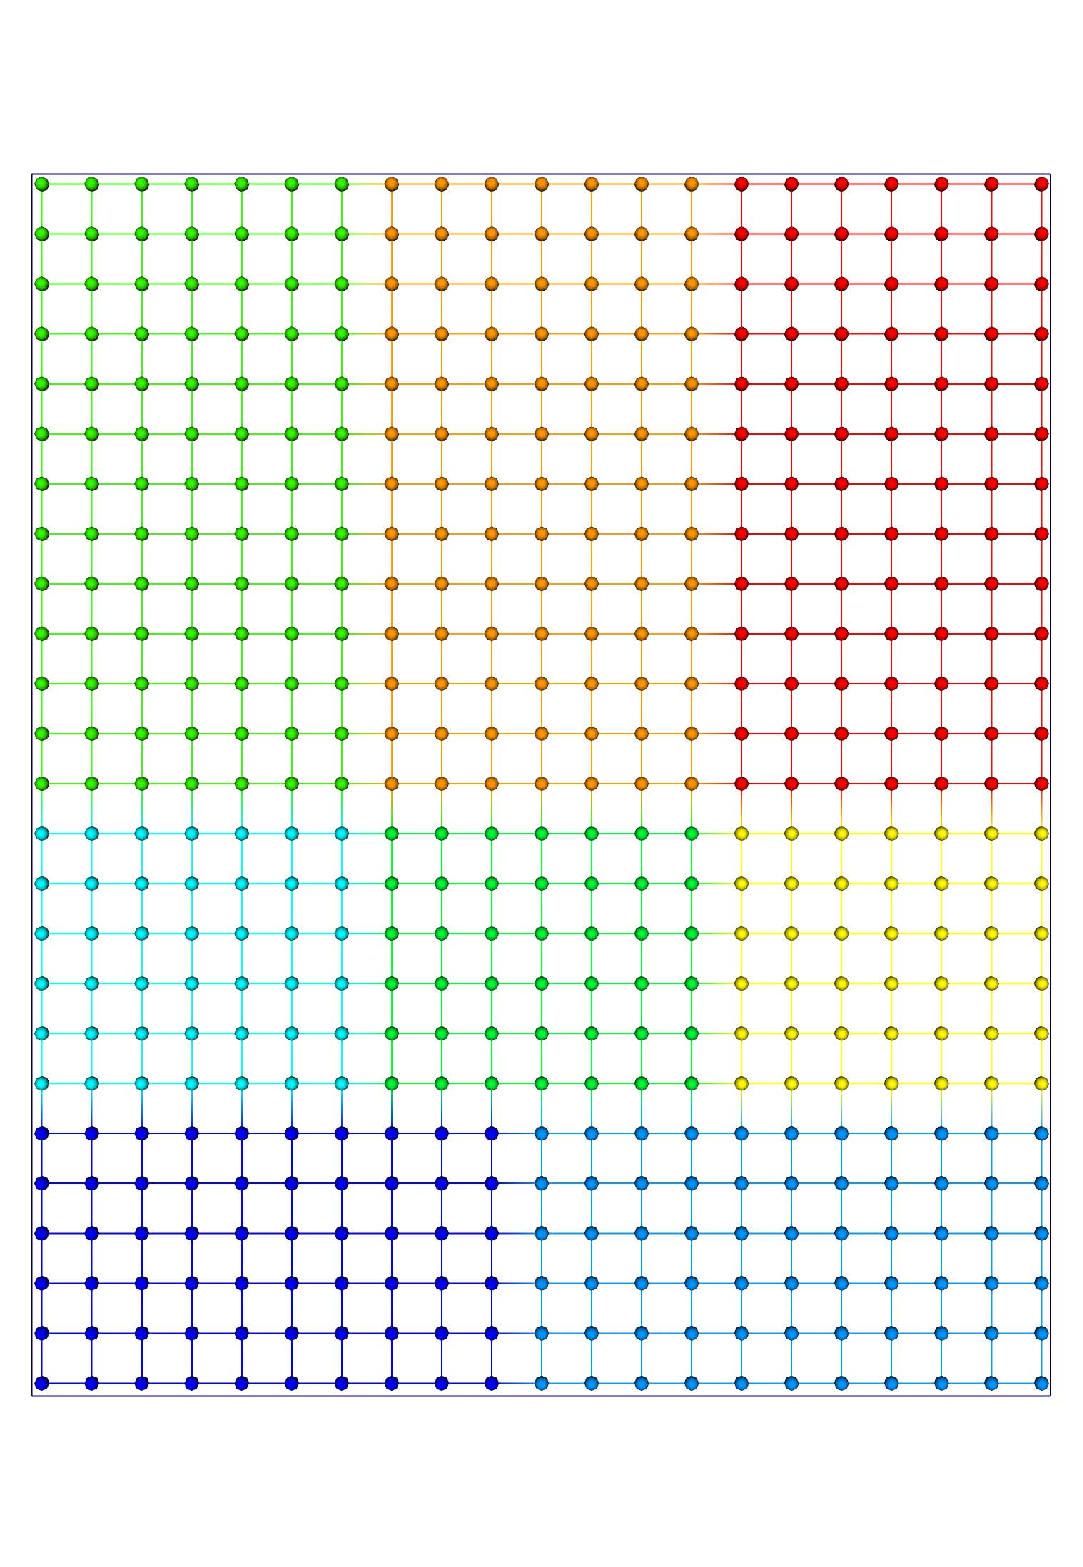
\includegraphics[width=3cm]{figures/partitioning/b_pow.pdf}}
    \subfigure[] {\label{fig:DifferentPartitioning-b}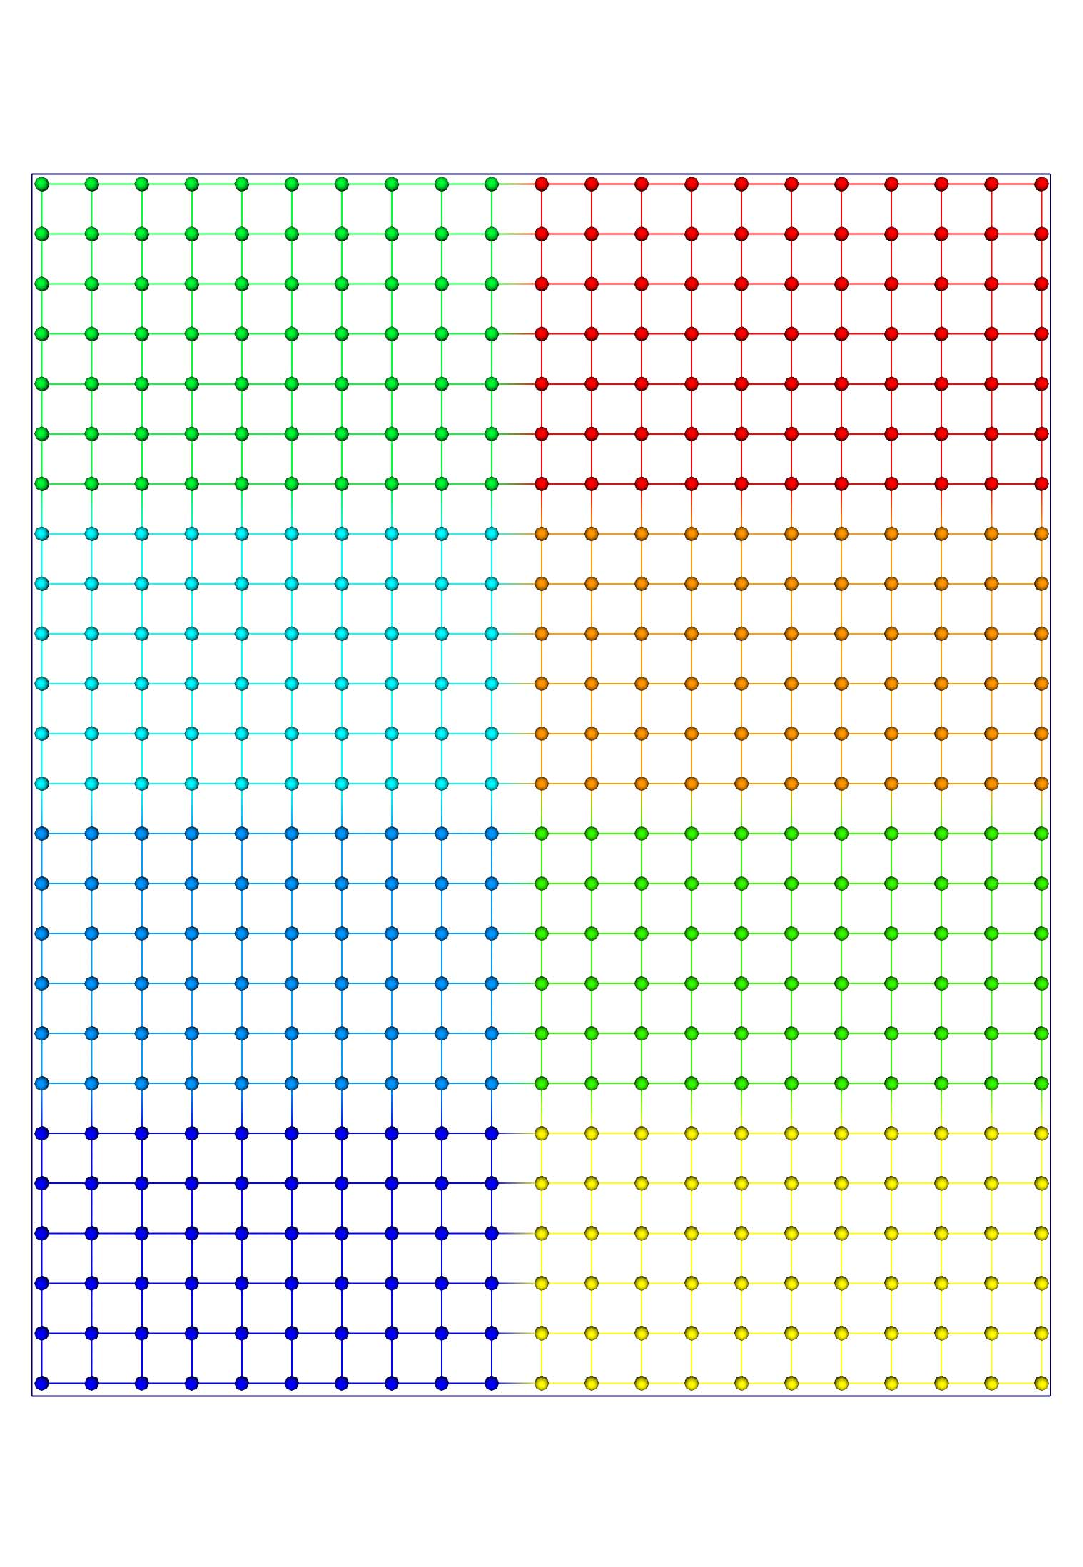
\includegraphics[width=3cm]{figures/partitioning/b_prime.pdf}}
    \subfigure[] {\label{fig:DifferentPartitioning-c}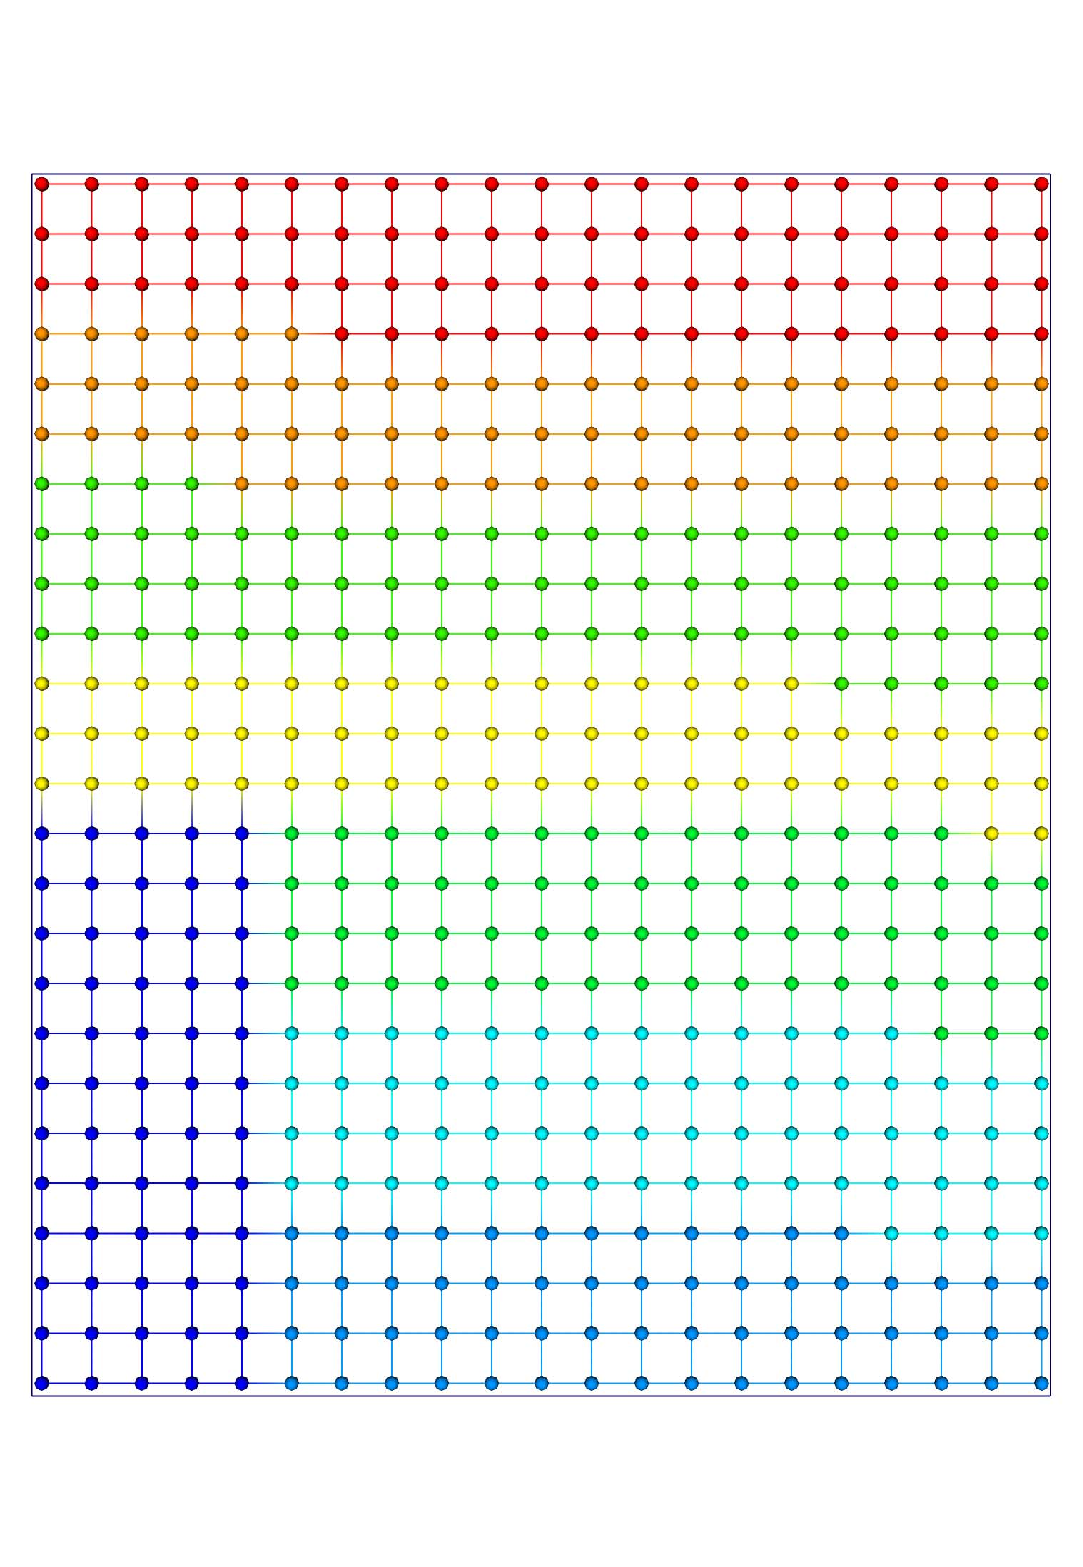
\includegraphics[width=3cm]{figures/partitioning/b_zol_geo.pdf}}
    \subfigure[] {\label{fig:DifferentPartitioning-d}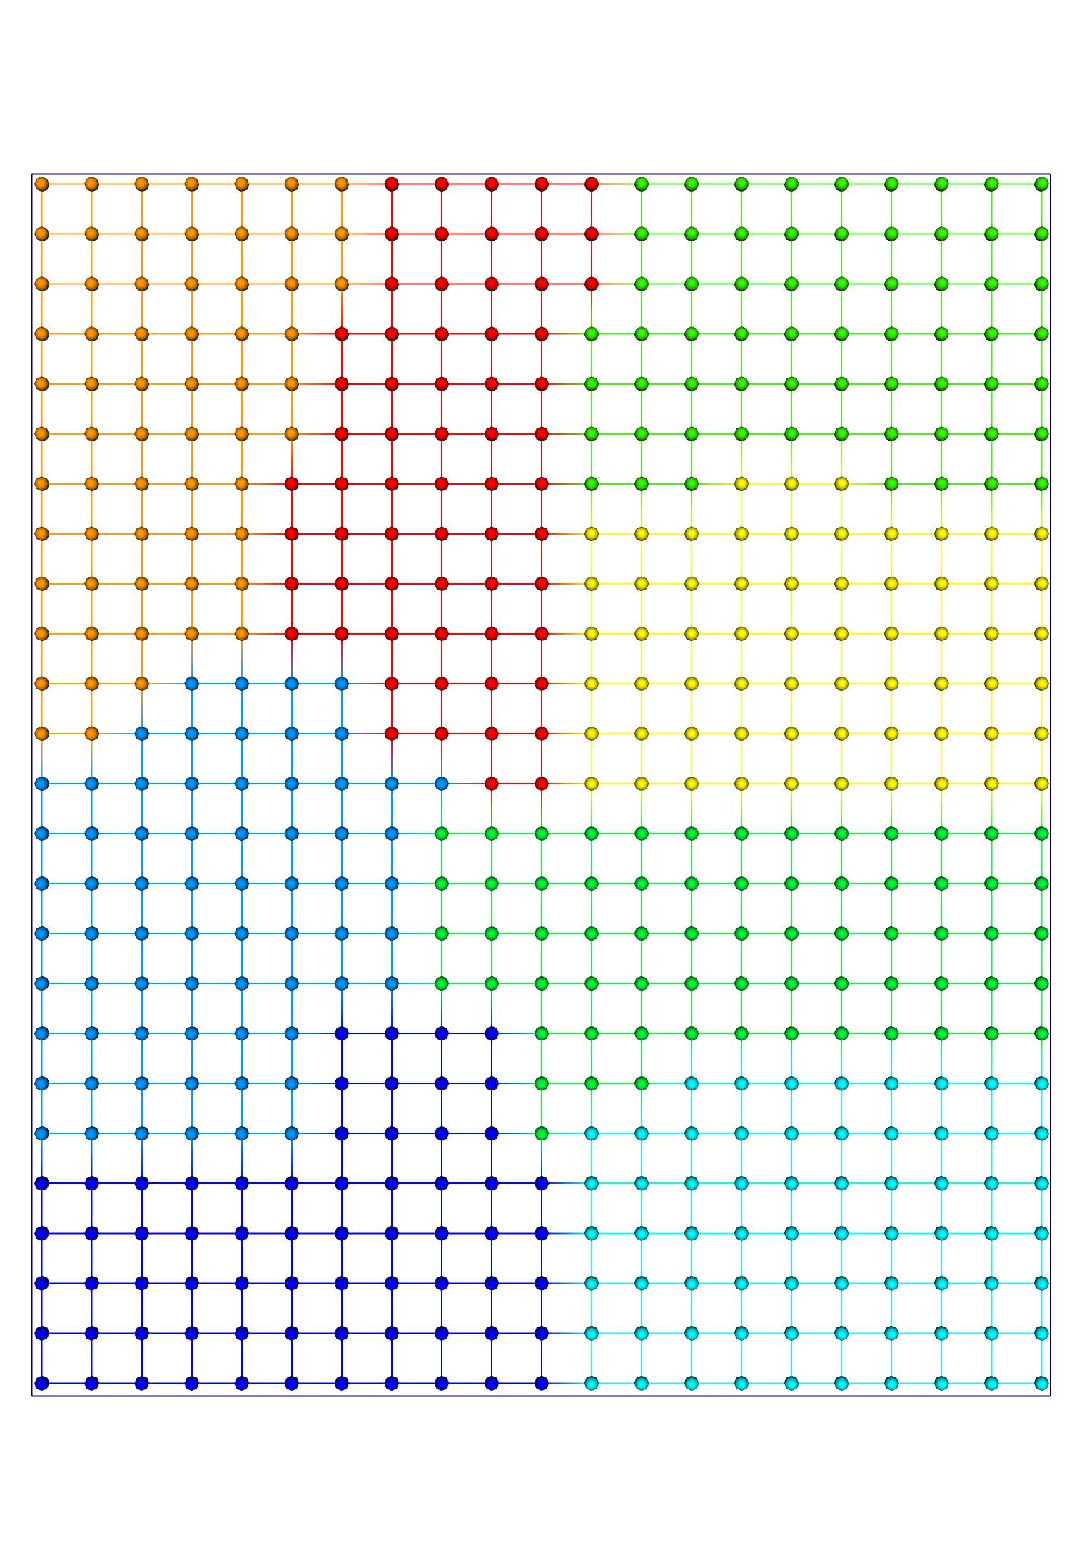
\includegraphics[width=3cm]{figures/partitioning/b_zol_hyp.pdf}}
  \end{center}
  \caption{Domain partitioning: (a) geometric simultaneous, (b) geometric sequential, (c) Zoltan geometric, (d) Zoltan hypergraph.}
  \label{fig:DifferentPartitioning}
\end{figure}

\begin{figure}
  \begin{center}
     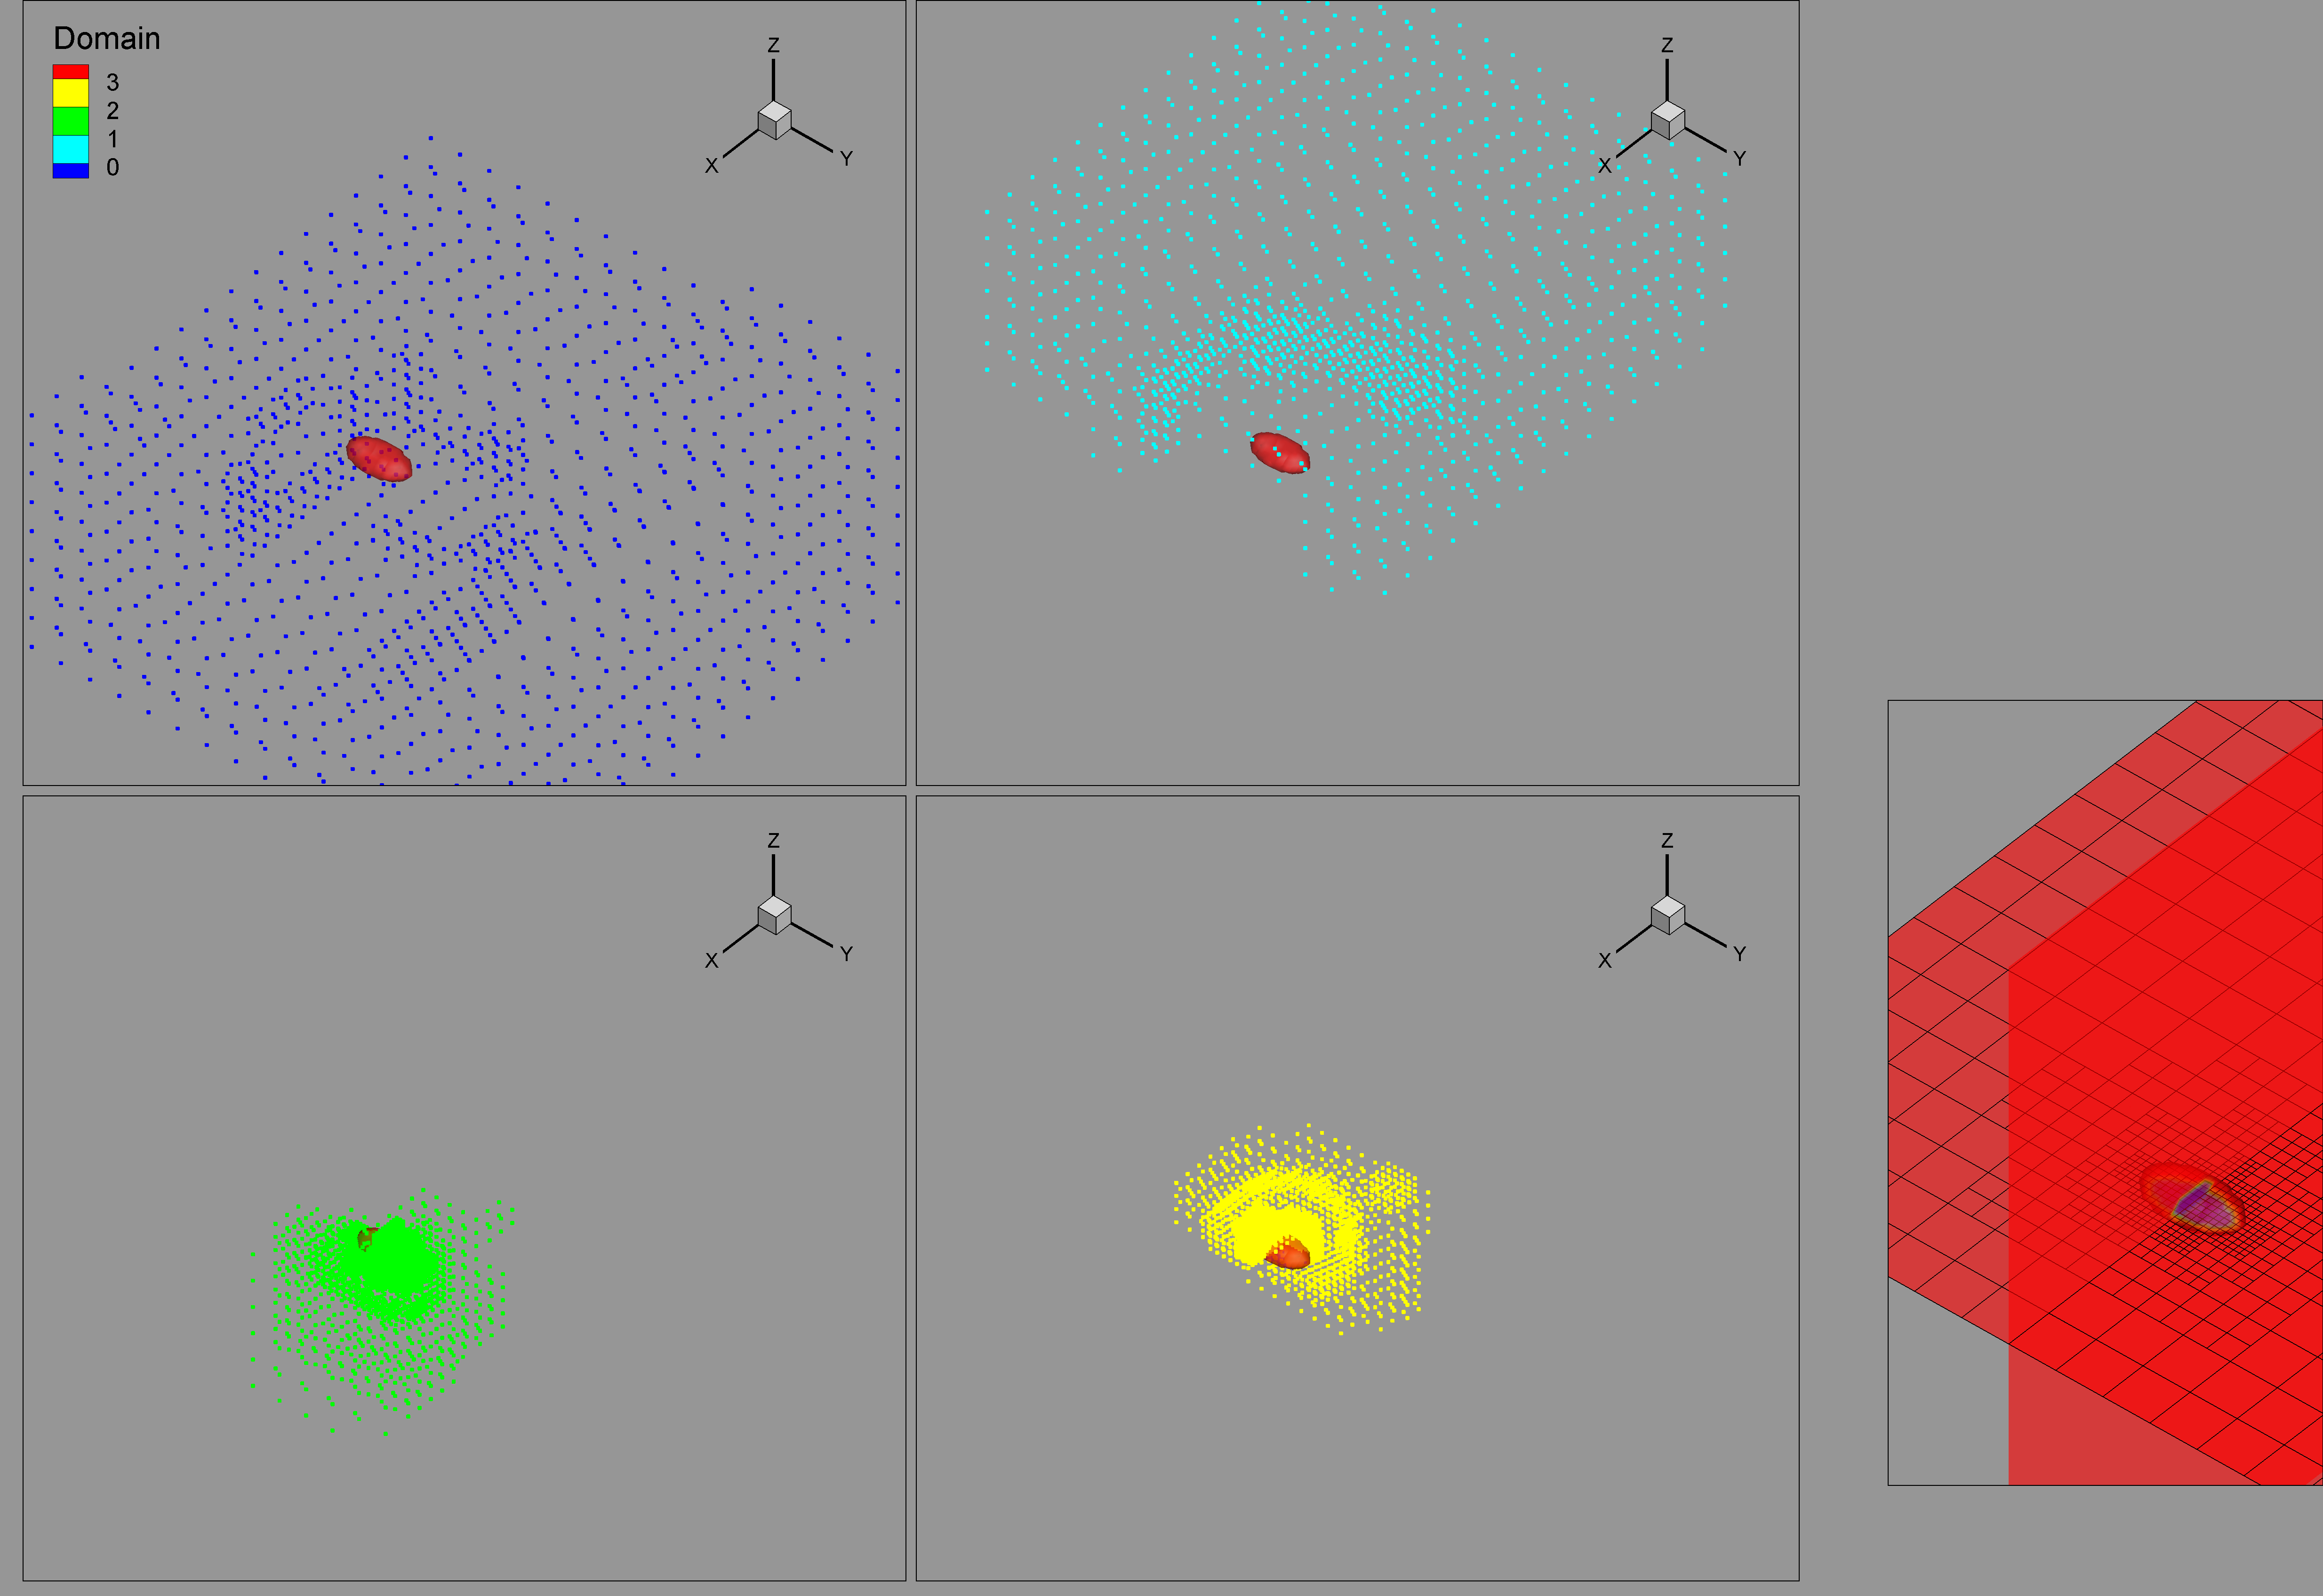
\includegraphics[width=10cm]{figures/domain_2.png}
  \end{center}
  \caption{ Dynamic Load balancing using Zoltan hypergraph domain partitioning for Convection-Diffusion of Rotating Ellipsoids.}
  \label{fig:ExamplePartitioning}
\end{figure}

\begin{figure}
\centerline{
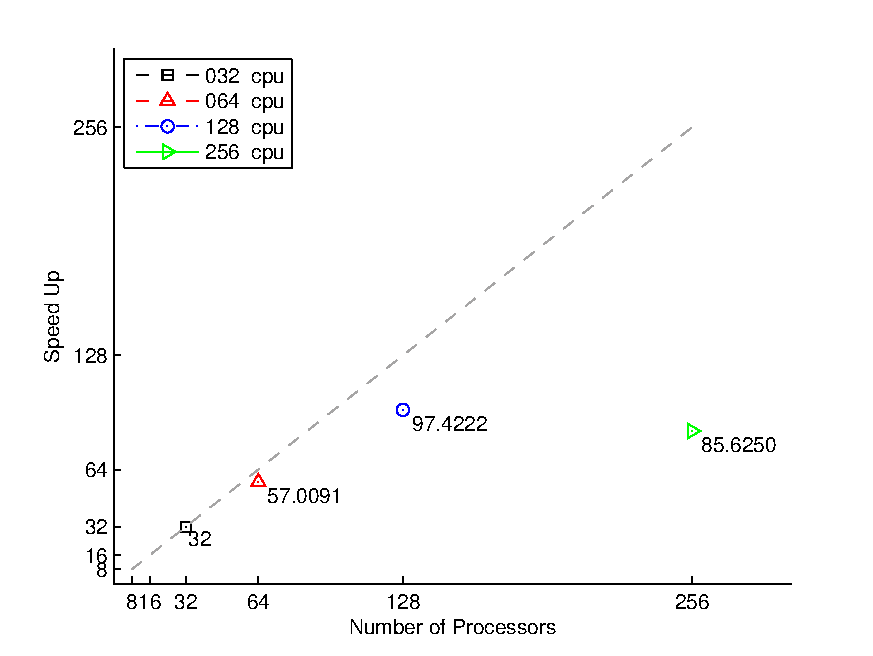
\includegraphics[width=10cm]{figures/SpeedUp_TimeIntegration_600.pdf}}
\caption{Parallel Speedup for CVS $\epsilon\rm{=0.2} \;\; \nu\rm{=0.015} \;\; C_f\rm{=6.\bar{6}} \;\; Re_{\lambda}\rm{=190} \;\; 1024^3$
         using geometric sequential partitioning.}
\label{fig:speedup}
\end{figure}

%
%2) parallel adaptive wavelet collocation method for the solution of partial differential equations.
%
%Two major building blocks are demonstrated in the current effort:
%1) variable thresholding which is the infrastructure of hybrid models within the context of wavelet-based methods;
%2) parallel adaptive wavelet based PDE solver. To the best of our knowledge, both parallel adaptive wavelet algorithm and hybrid wavelet-based models based on the notion of defining the thresholding-factor as a field variable are introduced for the first time.





  }
  \item \textbf{Solver Improvements} {

  A basic result of external flow application has shown in Chapter 3. Further progresses in the external flow studies has been captive of 
  some numerical instabilities initiated at the corner points of the domain which are caused by our current matrix-free solver. In an ongoing effort, through implementation of highly-scalable linear solvers of the Trilinos packages \cite{Trilinos-Tutorial, 1089021, Trilinos-Users-Guide, Trilinos-Dev-Guide-II, Trilinos-Dev-Guide, Trilinos-Overview}, it is planned to remove this limitation shortly.





  }
  \item \textbf{Lagrangian Averaged of Forcing} {

%\section{Lagrangian Averaged of Forcing}


Another ongoing investigation as discussed in the previous chapter is to track the forcing term itself within a Lagrangian frame so that
the forcing term inherits the history of the flow evolution, i.e., analogous to the FT2, the forcing is defined 
based on Lagrangian Averaged of Forcing, ${\mathcal I}_{F}$, 

%
%\begin{equation}
%       {\bareps[u]_i}  \;\;\;  \thicksim \;\;\;  \epsilon \;\;\; \& \;\;\; \Scl[u_i]
%\end{equation}

\begin{equation}
       {\rm  forcing_{term} } =
       \epsilon^{\rm old} \left( {\mathbf x}-\bareps[{\mathbf u}] \Delta t,t\right)
       \underbrace{C_{{\rm f}_{\epsilon}}}_{400}   %400 \;
       \frac 1 {\tau_{\epsilon}}
       \frac {1}{{\mathcal I}_{F}}
       ( \Pi - \varepsilon_{\rm res}  \frac {\rm Goal}{1-{\rm Goal}} ),
\end{equation}


where the Lagrangian Averaged of Forcing defined as the statistical average of the forcing, $F \left(\bx\left(\tau\right),\tau\right)$,
\begin{equation}
{\mathcal I}_{F}\left(\bx,t\right)  =
              {1 \over \tau_{\epsilon}} \int_{-\infty}^{t}
              %\int \!\!\!\int \!\!\!\int_{D}
              e^{\frac{\tau-t}{\tau_{\epsilon}}} %{\blue G \left( \by -\bx\left(\tau\right),\tau \right)}
                  F \left(\bx\left(\tau\right),\tau\right)
                  %M_{ij}\left(\bx\left(\tau\right),\tau\right) d \tau d \bV
                  d \tau.
\end{equation}

Similar to the threshold-factor, the Lagrangian representation of  $F \left(\bx\left(\tau\right),\tau\right)$, is tracked using the  Lagrangian Path-Line Diffusive Averaging approach:

\begin{equation}
        \label{eq:LagPathLineDiffAvg} \vspace*{3pt}
        \partial_{t}{\mathcal I}_{F}
        + \bareps[u]_j \partial_{x_j}{\mathcal I}_{F}
        = - \frac 1 \tau_{\epsilon} ( F_{\rm local} - {\mathcal I}_{F} )
        + \nu_{{\mathcal I}_{F}} \partial_{x_jx_j}^2{\mathcal I}_{F},
\end{equation}

where the local forcing is defined as follows:

\begin{equation}
       F_{\rm local} =  \Pi - \varepsilon_{\rm res}  \frac {\rm Goal}{1-{\rm Goal}}.
\end{equation}

Therefore, the forcing, $F \left(\bx\left(\tau\right),\tau\right)$, also follows the local flow structures as they evolve in space and time.

%\begin{equation}
%        F = {\rm Max}  \left| \Pi - \varepsilon_{\rm res}  \frac {\rm Goal}{1-{\rm Goal}} \right|
%\end{equation}
%
%
%\begin{equation}
%      {\rm  forcing_{term} } =
%                  \epsilon^{\rm old} \left( {\mathbf x}-\bareps[{\mathbf u}] \Delta t,t\right)
%                  \frac 1 {\tau_{\epsilon}}
%                  \frac {\Pi - \varepsilon_{\rm res}  \frac {\rm Goal}{1-{\rm Goal}}} {{\mathcal I}_{F}}
%\end{equation}





  }
  \item \emph{Stochastic SGS Models} {
  
  As discussed in Chapter 1, in the current implementation of the SCALES methodology, 
  only the effect of the ``minority deterministic coherent SGS modes''  on the ``deterministic most energetic coherent structures'' are modeled by the ``deterministic SGS models''. However, it is of great interest to be able to model 
  the effect of the ``majority stochastic incoherent SGS modes'' on the ``deterministic most energetic coherent structures'' as well by means of 
  ``stochastic SGS models''. The author feels in infancy stage of understanding the required mathematical background: theoretical/numerical Stochastic Partial Differential Equations (SPDE); however, he hopes he can at least make some preliminary progresses toward understanding the Stochastic SGS models and their implementation within SCALES framework.




  }
  \item \textbf{Uncertainty Quantification Studies} {
  
  It is said that among the the future directions of the computational sciences, main concern will be uncertainties issues.
  Keeping this in mind, another dream is to be able to fine-tune the deterministic SGS models based on the Uncertainty Quantification (UQ) concepts. Hence, it is hoped to be engaged in learning process of the UQ concepts and its possible advantages in instantaneous corrections/adjustments of the SGS models. The UQ based adjustment of the time-relaxation-parameter and forcing-term of the threshold-factor Lagrangian evolution, as well as UQ based adjustment of hybrid model transition algorithm (when/where to switch among WDNS/CVS/SCALES) are also on the wish-list.
  
  
  }
\end{itemize} 

  
  
  
\vspace{50pt}

Finally, in words of Marcel Lesieur \cite{Book_Turbulence_Lesieur},
\begin{quotation}
It might finally happen that this would be only a necessary transition stage toward the definition of new fluid dynamical concepts
which would render obsolete and useless the complicated analytical and numerical techniques which helped create them.
\end{quotation}
